\subsection{Surface Quasi-Geostrophic Turbulence}
\label{subsec:sqg}

Our goal in this study is to show how relatively simplified RNNs can be used to
predict turbulent Geophysical Fluid Dynamics, while avoiding the complications
associated with realistic atmosphere or ocean GCMs.
Therefore, we aim to emulate a numerical model for Surface Quasi-Geostrophic
(SQG) turbulence as outlined by \citet{tulloch_note_2009}.
The model is formulated based on the nonlinear Eady problem
\citep{eady_long_1949}, following \citet{blumen_uniform_1978-1}.
The model simulates turbulence
on an $f$ plane with uniform stratification and shear, and bounded by rigid
surfaces $H=10$~km apart.
The motion is determined entirely by temperature advection on the boundaries
$z=\{0,H\}$ as follows,
\begin{equation*}
    \dfrac{\partial \hat{\theta}}{\partial t} +
    \hat{J}(\hat{\psi}, \hat{\theta}) + ik\left(U \hat{\theta} +
        \hat{\psi}\dfrac{\partial \Theta}{\partial y}\right)
    = 0 \qquad z = 0, H \, .
\end{equation*}
Here, hatted variables denote spectral components, $\hat{J}$ is the Jacobian in
spectral space, and the temperature streamfunction is
\begin{equation*}
    \hat{\psi}(z,t) = \dfrac{H}{\mu\sinh\mu}
    \left[ \cosh\left(\mu\dfrac{z}{H}\right) \hat{\theta}(H,t)
        - \cosh\left(\mu\dfrac{z-H}{H}\right) \hat{\theta}(0,t)
    \right]\, ,
\end{equation*}
with $\mu = |\mathbf{K}| NH/f$ as the nondimensional wavenumber.
We note that this model produces a -5/3 spectrum without any break,
as is expected in Eady turbulence.
For more details, see \citep{tulloch_note_2009}.


\begin{figure}
    \centering
    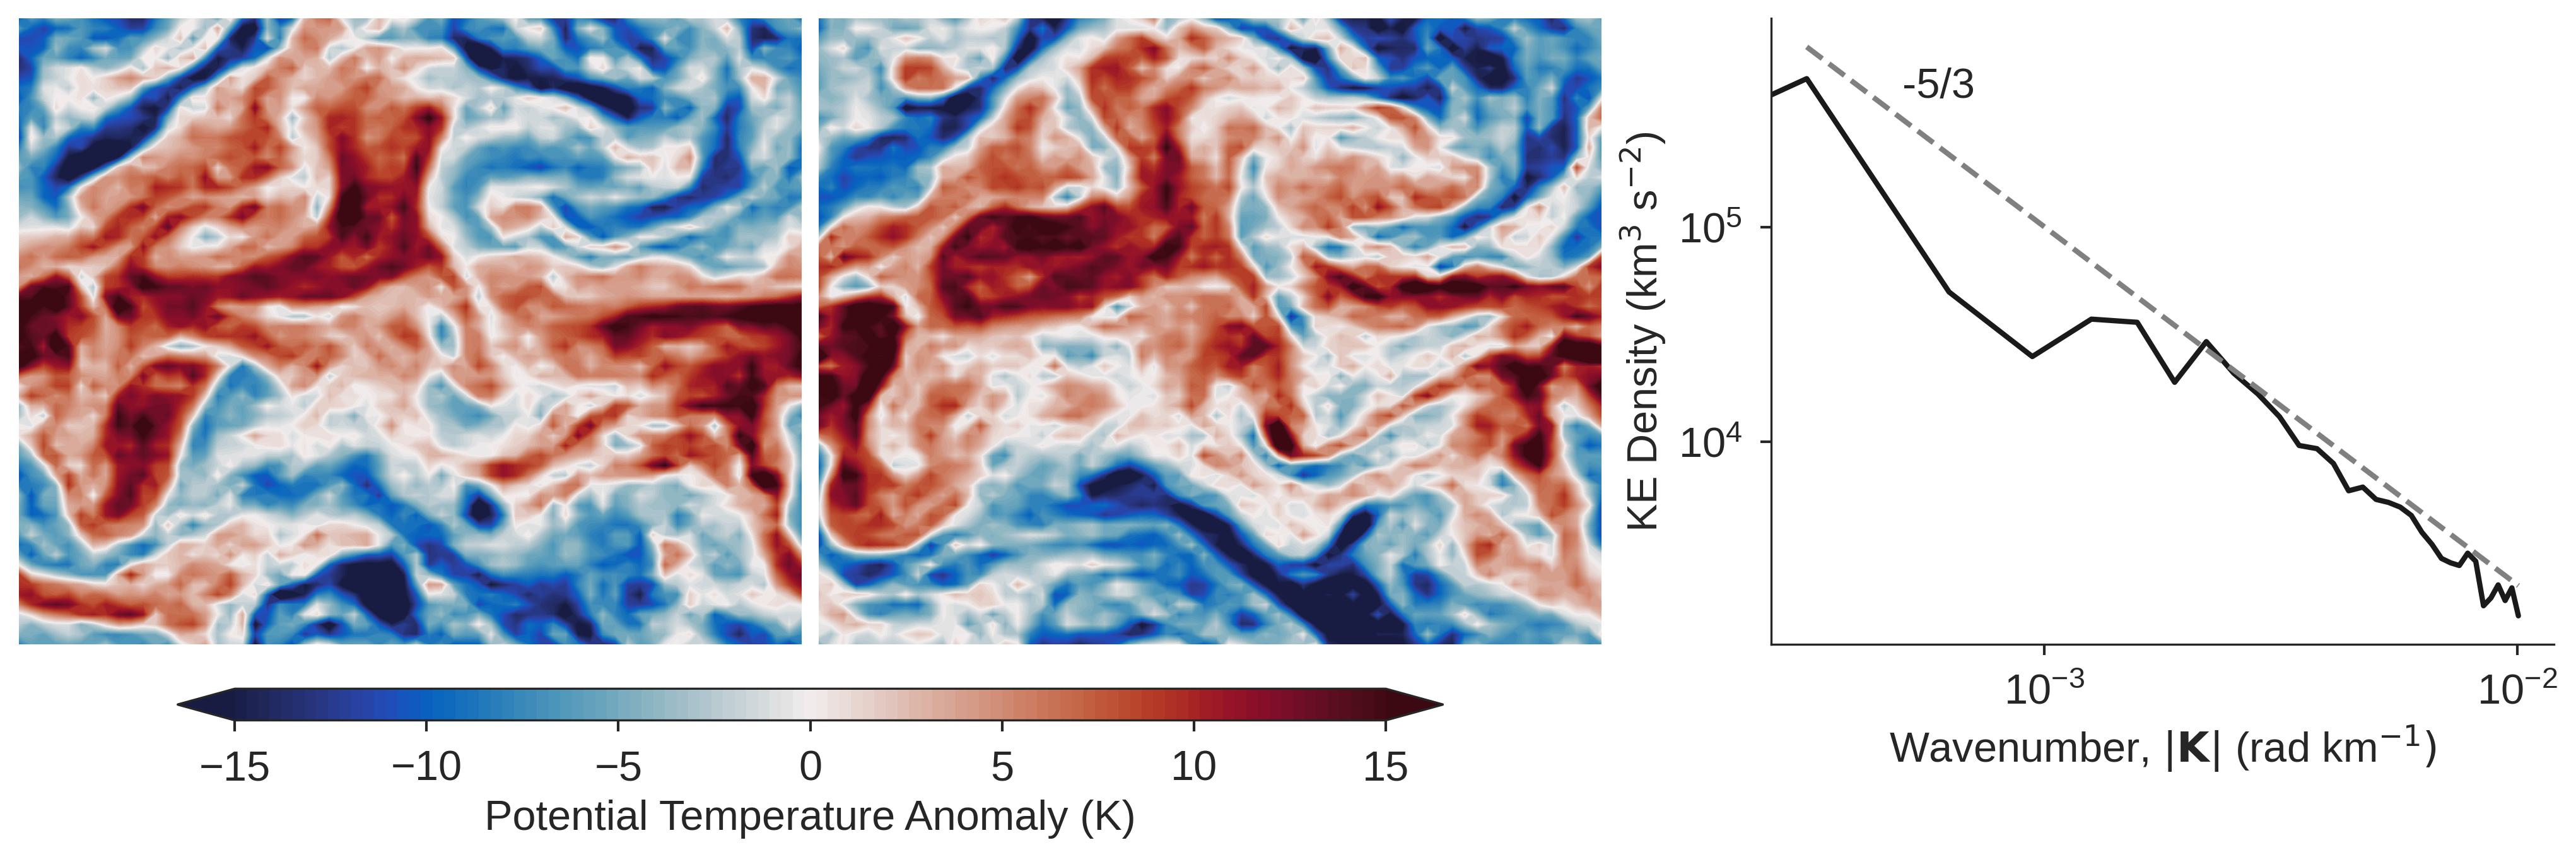
\includegraphics[width=\textwidth]{../figures/sqg_reference_plot.jpg}
    \caption{Reference plot}
    \label{fig:sqg-reference}
\end{figure}

%\subsection{Training, Validation, and Testing Datasets}

The model is discretized in space with $N_x = N_y = 64$, corresponding to
grid spacing of \red{XX}~km, although we recall that the spectral coefficients
are used to evolve the model forward in time.
The model timestep is $\Delta t=5$~minutes.
To generate datsets for the RNNs, we initialize the surface layer with Gaussian,
i.i.d. noise: $\theta(z=0, t=t_0) \sim \mathcal{N}(0, 100$~K), and the top layer
with $\theta(z=H, t=t_0) = 2000 \sin^{40}(x/2)\sin^{20}(y)$.
\todo{Why TF do we do this again?}
We spinup the model for 360~days, which we define as one model year.
The spinup period is discarded, and we store the following 15~years for training
and validation data.
We then evaluate and discard a 5~year transient period, and store the final
10~years for testing.
